\documentclass[tikz,border=10pt]{standalone}
\usepackage{pgfplots}
\usepgfplotslibrary{fillbetween}
\pgfplotsset{compat=1.18}

\begin{document}

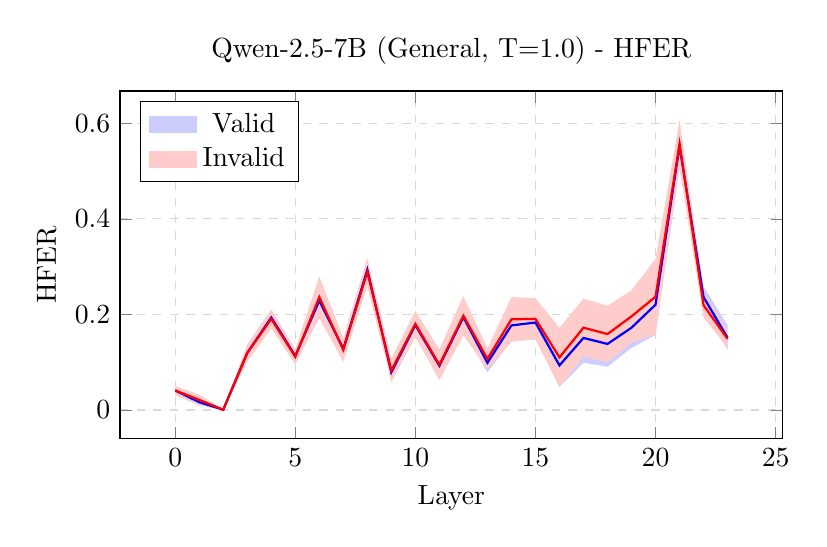
\begin{tikzpicture}
\pgfplotstableread[row sep=newline, col sep=comma]{
layer,v_mean,v_std,i_mean,i_std,v_upper,v_lower,i_upper,i_lower

0,0.0408783689092256,0.00938553034090295,0.04084395966492589,0.009319505062307365,0.05026389925012855,0.031492838568322655,0.05016346472723326,0.031524454602618525

1,0.016265811076951412,0.006499986678596211,0.021150966524146445,0.010956575231903342,0.022765797755547622,0.009765824398355202,0.03210754175604979,0.010194391292243104

2,0.00041958982154407154,0.0002617494266145712,0.0005013543456394542,0.00024312270401573256,0.0006813392481586427,0.00015784039492950036,0.0007444770496551868,0.00025823164162372164

3,0.11931395177778441,0.014090330923418578,0.11917919665575023,0.01835621807225283,0.133404282701203,0.10522362085436583,0.13753541472800307,0.1008229785834974

4,0.1934132677944083,0.015170351366782069,0.190696466093262,0.01995242498136682,0.20858361916119036,0.1782429164276262,0.2106488910746288,0.17074404111189517

5,0.11292666451711399,0.011544397251769381,0.11131672592212753,0.015959915394080794,0.12447106176888337,0.1013822672653446,0.12727664131620833,0.09535681052804673

6,0.22885339883597275,0.023567482484236554,0.2361032764116923,0.043564685786066586,0.2524208813202093,0.2052859163517362,0.27966796219775886,0.1925385906256257

7,0.12793176680019022,0.01467174820944855,0.12575457834949091,0.024924808884035463,0.14260351500963878,0.11326001859074167,0.15067938723352636,0.10082976946545545

8,0.2933604083955288,0.01580070522099113,0.2888143826276064,0.029105398933909447,0.30916111361651993,0.27755970317453765,0.31791978156151585,0.25970898369369694

9,0.07875870378982075,0.020064463656285062,0.0827362053096294,0.024534883309267175,0.09882316744610581,0.05869424013353569,0.10727108861889657,0.058201322000362224

10,0.1775626636257297,0.017732945296785547,0.18015637993812553,0.027456832559599353,0.19529560892251524,0.15982971832894416,0.20761321249772488,0.15269954737852617

11,0.0924202280707265,0.023165862514982705,0.09459596360102292,0.03240261484349395,0.1155860905857092,0.0692543655557438,0.12699857844451687,0.062193348757528966

12,0.1939904550580602,0.026521338135132518,0.19716689921915523,0.04090425211103989,0.22051179319319272,0.16746911692292768,0.23807115133019513,0.15626264710811533

13,0.09869286604225631,0.020009133307242775,0.10668873554095622,0.022153080028346088,0.11870199934949908,0.07868373273501354,0.1288418155693023,0.08453565551261014

14,0.1768942790988244,0.03237407750393591,0.18958412421246365,0.0467051710791263,0.20926835660276033,0.1445202015948885,0.23628929529158996,0.14287895313333734

15,0.1829773509188702,0.02937951235176806,0.19066735481222463,0.04322471923526686,0.21235686327063827,0.15359783856710216,0.2338920740474915,0.14744263557695778

16,0.09320930641536646,0.044964474003861006,0.10991249644818402,0.062360190875136404,0.13817378041922745,0.04824483241150545,0.1722726873233204,0.04755230557304761

17,0.15071438821522812,0.051893606652435684,0.17215956312914685,0.06082147082970348,0.2026079948676638,0.09882078156279243,0.23298103395885034,0.11133809229944336

18,0.13813741887478448,0.04771295580687376,0.1588539499789476,0.05923209534808252,0.18585037468165824,0.09042446306791072,0.21808604532703013,0.09962185463086509

19,0.1721344972519498,0.04225394160843555,0.19581735009948406,0.05464693868281213,0.21438843886038533,0.12988055564351425,0.2504642887822962,0.14117041141667191

20,0.22024432501118435,0.06344631393212988,0.23691477626562119,0.07920052545273625,0.28369063894331426,0.15679801107905447,0.31611530171835744,0.15771425081288493

21,0.552284479925507,0.04651376525208457,0.557408389945825,0.04949271255819196,0.5987982451775916,0.5057707146734224,0.606901102504017,0.507915677387633

22,0.23602140930138135,0.02227896496315153,0.21921562838057676,0.025391662949768846,0.2583003742645329,0.2137424443382298,0.24460729133034562,0.1938239654308079

23,0.15104836166689267,0.0256329415031575,0.14849620374540484,0.018899854718081026,0.17668130317005018,0.12541542016373516,0.16739605846348588,0.1295963490273238

}\mydata

\begin{axis}[
    width=10cm, height=6cm,
    xlabel={Layer},
    ylabel={HFER},
    title={Qwen-2.5-7B (General, T=1.0) - HFER},
    legend pos=north west,
    grid=major,
    grid style={dashed, gray!30}
]

\addplot [name path=v_upper, draw=none, forget plot] table [x=layer, y=v_upper] {\mydata};
\addplot [name path=v_lower, draw=none, forget plot] table [x=layer, y=v_lower] {\mydata};
\addplot [blue!20] fill between [of=v_upper and v_lower];

\addplot [name path=i_upper, draw=none, forget plot] table [x=layer, y=i_upper] {\mydata};
\addplot [name path=i_lower, draw=none, forget plot] table [x=layer, y=i_lower] {\mydata};
\addplot [red!20] fill between [of=i_upper and i_lower];

\addplot [blue, thick] table [x=layer, y=v_mean] {\mydata};
\addlegendentry{Valid}
\addplot [red, thick] table [x=layer, y=i_mean] {\mydata};
\addlegendentry{Invalid}

\end{axis}
\end{tikzpicture}
\end{document}
